\usepackage{amsmath}

\chapter{Work description}
\label{cap:descripcionTrabajo}

% #1 = tikz options (optional)
% #2 = total width (e.g. 7cm)
% #3 = height      (e.g. 0.5cm)
% #4 = wins
% #5 = draws
% #6 = losses
\newcommand{\ResultBar}[6][]{%
  \begingroup
  % compute totals & scaled lengths
  \pgfmathsetmacro{\TotalGames}{#4 + #5 + #6}%
  \pgfmathsetlengthmacro{\TotalWidth}{#2}%
  \pgfmathsetlengthmacro{\BarHeight}{#3}%
  \pgfmathsetlengthmacro{\WinWidth}{#4/\TotalGames*\TotalWidth}%
  \pgfmathsetlengthmacro{\DrawWidth}{#5/\TotalGames*\TotalWidth}%
  \pgfmathsetlengthmacro{\LossWidth}{#6/\TotalGames*\TotalWidth}%
  %
  \begin{tikzpicture}[#1]
    % coloured segments
    \fill[green!70!black] (0,0) rectangle (\WinWidth,\BarHeight);
    \fill[gray] (\WinWidth,0) rectangle (\WinWidth+\DrawWidth,\BarHeight);
    \fill[red!70!black] (\WinWidth+\DrawWidth,0)
                       rectangle (\WinWidth+\DrawWidth+\LossWidth,\BarHeight);
    % outer border
    \draw (0,0) rectangle (\TotalWidth,\BarHeight);
    % labels above each segment
    \node[font=\footnotesize] at (\WinWidth/2,1.4*\BarHeight)
      {\textbf{#4} wins};
    \node[font=\footnotesize] at (\WinWidth + \DrawWidth/2,1.4*\BarHeight)
      {\textbf{#5} draws};
    \node[font=\footnotesize] at (\WinWidth+\DrawWidth + \LossWidth/2,1.4*\BarHeight)
      {\textbf{#6} losses};
  \end{tikzpicture}%
  \endgroup
}

We designed a simple structure to organize all the scripts. As we are implementing different versions of the engine, there are specific modules that are compulsory to have well distinguished and possibly selected between them. Those modules are presented in the following Section~\ref{sec:modules}.

\vspace{1em}

\noindent Next, the key point is how to represent each required structure, including the board, chess pieces, precomputed tables, transposition tables, etc., as discussed in Section~\ref{sec:code}.

\section{Modules}
\label{sec:modules}

Each module is responsible for a specific aspect of the chess engine's functionality. The good part about this modular design is that it ensures clarity, maintainability, and the ability to test and improve individual components independently even more so when it comes to development with more people.

\subsection{Board}

\noindent This module handles the representation of the chessboard, as previously mentioned in Section~\ref{sec:board}, and the state of the game. It includes:
\begin{itemize}
    \item Representation of the chessboard with its pieces using bitboards for efficiency.
    \item Functions to make and unmake moves, including special moves like castling and en passant.
    \item Updating game state variables, such as castling rights or the half-move counter.
\end{itemize}

\noindent This module is vital, as it provides the data structures and operations required by other modules.

\subsection{The core, search algorithm}

The core of the chess engine is its search algorithm; alpha-beta pruning is an\\
improved version of the minimax algorithm. The entire game tree is generated\\
up to a selected maximum depth. At each node, the next player evaluates the\\
position; White tries to maximize the evaluation, while Black tries to minimize it.\\
During execution,the values of alpha (the best evaluation so far for MAX, hence\\
choosing the highest value) and beta (the best evaluation so far for MIN, hence\\
choosing the lowest value) are updated. Pruning is performed when a branch of the\\
tree is detected as irrelevant because the evaluation being examined is worse than\\
the current value of alpha or beta for MAX or MIN, respectively.\\

TODO: insert diagram of alpha beta pruning\\

Therefore, the following events happen at each node of the tree:\\

\begin{itemize}
    \item \textbf{Check if we are at an end node:} because a checkmate occurs, a draw by triple repetition, the 50-move rule, or because we have reached the maximum selected depth.
    
    \item \textbf{Evaluate the position:} A positive value (+) means that White has an advantage, and a negative value (-) means that Black has an advantage. A limit is set that represents mate in one; we have arbitrarily chosen 3,200,000.
    
    \item \textbf{Generate legal moves:} create a list of every possible legal move in the position.
    
    \item \textbf{Order the legal moves:} from greatest to least intuition of being the best move for the position. The sooner we explore the best move, the more branches of the tree will be pruned.
    
    \item \textbf{Explore each of the legal moves:} from the position in order, update the evaluation, the value of alpha and beta, and check if we can perform pruning.
\end{itemize}

\subsection{search: iterative deepening}

At what depth do we decide to search? Actually, the simplest thing is to perform\\
an infinite search, first searching at depth 1, then 2, then 3... to infinity.\\
The engine will update the evaluation and the best move for the position with\\
each iteration. Simply by signaling "Stop," the search will stop.\\

TO DO : iterative deepening image\\

\subsection{search: horizon effect, quiescence search}

What happens if, upon reaching maximum depth, we evaluate the position in the\\
middle of a piece exchange? For example, if a queen captures a pawn. It will\\
seem like we've won a pawn, but on the next move, another pawn captures the\\
queen, and now we lose a queen. This is known as the horizon effect. To avoid\\
this, when we reach the end of the tree at maximum depth, we must extend the\\
search to include only piece captures. This is known as quiescence search.\\

The purpose of this search is only to stop the search and evaluate quiet\\
positions, where there is no capture or tactical movement.\\

TO DO : quiescence search  image\\

\ldots

\subsection{Evaluation}

TODO: (this section could be merged with the previous evaluation explanation) \\

The most obvious way to evaluate a chess position is by counting the\\
pieces on the board. We've assumed that the pawn is worth 100 points,\\
the knight 320, the bishop 330, the rook 500, and the queen 950. Black's\\
pieces will have a negative value. Therefore, the evaluation of a position\\
is the sum of the values of all the pieces.\\

This approach is very naive for several reasons: pieces are stronger on\\
different squares on the board. For example, a knight in a corner only\\
attacks 2 squares, while in the center of the board it attacks 8 squares.\\

TODO: insert diagram of knight moves in square vs in the center\\

To reflect this characteristic, we add a bonus to the value of each piece\\
depending on the square it occupies; we use the so-called Piece Square Tables.\\
This is the bishop's PST:\\

TODO: insert diagram of bishop piece square table\\

This evaluation still ignores the fact that a chess game is divided into three\\
phases: opening, middlegame, and endgame. The current approach is useful in the\\
opening and middlegame because it rewards developing pieces and placing them on\\
squares where they maximize their potential. The problem arises in endgames, where\\
it's often a good idea to be much more aggressive, seeking to push pawns to their\\
promotion squares. Furthermore, the king becomes more important because there are\\
fewer pieces on the board, allowing him to join the attack without compromising\\
his security.\\

We can perform a dynamic evaluation (tampering evaluation). Evaluate twice, once\\
as if we were in the middlegame and once as if we were in the endgame. The final\\
evaluation will be the sum of both, but each with a different weight. To do this,\\
we calculate the middlegame percentage (24 pieces means 100\% middlegame) and the\\
endgame percentage (0 pieces = 100\% endgame).\\

TODO: insert diagram of pawn PST in middlegame and in the endgame to compare\\

\begin{align*}
\text{Evaluation} &= middlegame\% \cdot eval_middlegame + endgame\% \cdot eval_endgame \\
\end{align*}

\ldots

\subsection{Move generator}

TODO: add citation https://peterellisjones.com/posts/generating-legal-chess-moves-efficiently/ \\

Calculating the legal moves in a chess position is a more difficult and tedious task than it might seem, mainly due to the unintuitive rules of en passant and castling, and it is also difficult to restrict the moves of pinned pieces.

To create an efficient move generator, we will represent a chess position using bitboards. A board is made up of 64 squares; a bitboard is a 64-bit variable in which each bit represents whether a square is occupied or not. We have one bitboard for each type of piece to represent a position. For example, this is the white pawn bitboard in the initial position.

TODO: add bitboard image (this section could be merged with the previous bitboard explanation) \\

\begin{itemize}
    \item \textbf{Bitboards make movement generation more efficient:} because we can move pieces and calculate their attacks using arithmetic-logical operations and bit masks.

    \item \textbf{The steps to generate legal movements efficiently are the following:}
    \begin{itemize}
        \item \textbf{Calculate the bitboard of attacked squares:} by the waiting side.
        \item \textbf{Calculate bitboard dof pinned pieces.}
        \item \textbf{Generate the legal moves:} of each piece of the side whose turn it is, knowing that the king cannot move to any attacked square and that pinned pieces can only move in the direction of the pin.
        \item \textbf{Generate the special legal moves:} like en passant and castling.
    \end{itemize}
\end{itemize}
  

\ldots

\subsection{Move ordering}

Order the legal moves from most to least likely to be the best move in the\\
position. The sooner we explore the best move, the more branches of the tree\\
will be pruned. To do this, we use the MVV-LVA heuristic (most valuable victim,\\
least valuable aggressor). We give higher scores to capturing a low-value piece\\
over a higher-value piece. Capturing a queen with a pawn scores highly. We also\\
give a bonus to piece promotions.\\

TO DO: insert move ordering image\\

\subsubsection{Killer moves}

A \textbf{Killer Move} is a non-capturing (quiet) move that previously caused a beta-cutoff during the search in a sibling node or any other branch at the same depth in the game tree.

\begin{itemize}
  \item These moves are often strong candidates, as they have previously led to pruning in similar positions.
  \item Promoting them early in the move ordering increases the chances of early cutoffs, which improves search efficiency.
\end{itemize}

To take advantage of this heuristic:
\begin{itemize}
  \item We store up to two killer moves for each search depth.
  \item During move ordering, these killer moves are given a bonus score, allowing them to be explored before other quiet moves.
\end{itemize}

\ldots

\section{Improvements}

\ldots

\subsection{Transposition Table}

The basic implementation of the chess engine generates a large amount of\\
redundant calculations due to transpositions: situations in which the same\\
board position is reached through different sequences of moves in the game tree.\\

TODO insert transposition image.\\

Taking advantage of the concept of dynamic programming, we're going to create a\\
look-up table of chess positions and its evaluation. So if we encounter the same\\
position again, the evaluation is already precalculated. There's a problem: how\\
much space does the look-up table take up if there are an astronomical amount
of chess positions? What we can do is assign a hash to each position and make the\\
table index the last bits of the hash. The larger the table, the less likely access\\
collisions will be. We also want a hash that's fast to calculate and has\\
collision-reducing properties; for this, we'll use the Zobrist hashing technique.\\

\subsubsection{Zobrist Hashing}

Zobrist Hashing is a technique to transform a board position of arbitrary size\\
into a number of a set length, with an equal distribution over all possible\\
numbers, invented by Albert Zobrist.\\

To generate a 64-bit hash for a position, the following steps are followed:\\

\begin{itemize}
  \item There are 12 different types of chess pieces. For each of the 64 squares on the board, we generate 12 random 64-bit integers. That is, each piece-square combination is assigned a unique random value. This initialization step is performed only once when the program starts.
  
  \item The hash value for a given position is computed by performing the XOR operation between the hash accumulator and the random value corresponding to each piece on its square.
  
  \item In addition to the pieces, we also include:
  \begin{itemize}
    \item A random value for the side to move (white or black),
    \item One random value per square to account for the possibility of an \textit{en passant} capture.
  \end{itemize}
  
  \item These random values are carefully chosen so that even slightly different positions produce very different hash values. This greatly reduces the chance of collisions.
  
  \item The XOR operation is used not only because it is computationally inexpensive, but also because it is reversible. This means that when a move is made or undone, we can update the hash incrementally by applying XOR only to the affected squares, without needing to recompute the entire hash.
\end{itemize}

\subsubsection{Table Entry}

Each entry in the transposition table stores the following information:

\begin{itemize}
  \item \textbf{Zobrist Hash:} The full 64-bit hash of the position. This is used to verify that the entry corresponds to the current position and to detect possible index collisions in the table.
  
  \item \textbf{Evaluation:} The numerical evaluation of the position, as computed by the evaluation function.
  
  \item \textbf{Depth:} The depth at which the evaluation was calculated. A deeper search could potentially yield a more accurate evaluation, so this value helps determine whether a new evaluation should overwrite the existing one.
  
  \item \textbf{Node Type:} Indicates the type of node stored:
  \begin{itemize}
    \item \texttt{EXACT} the evaluation is precise for this position.
    \item \texttt{UPPERBOUND} the evaluation is an upper bound, typically resulting from an alpha cutoff.
    \item \texttt{LOWERBOUND} the evaluation is a lower bound, typically resulting from a beta cutoff.
  \end{itemize}
\end{itemize}

TODO: insertar imagen zobrist hashing

\subsubsection{Collisions}

As discussed earlier, index collisions in the transposition table are handled\\
by verifying the full Zobrist hash stored in the entry. However, it is still\\
theoretically possible for a full hash collision to occur, that is two\\
different positions producing the same hash.\\

This scenario is extremely rare. With 64-bit hashes, there are $2^{64}$ possible\\
unique values, which is more than sufficient for practical purposes.\\
In the unlikely event of a true hash collision, it could result in an\\
incorrect evaluation being reused for a different position.\\

\subsubsection{Analysis}

To evaluate the improvement introduced by the transposition table, we conducted\\
a 100-game tournament against the basic version of the engine. We selected 50\\
random starting positions from an opening book and played each position twice,\\
alternating colors to ensure fairness. Each bot has 4 seconds to think per move.\\

\textbf{64MB Transposition Table bot vs basic bot}\\
\ResultBar{15cm}{0.5cm}{46}{22}{32}
\medskip

We see a substantial improvement by adding the transposition table\\
with 46 wins versus 32 losses.\\

\ldots

\subsection{move generator with Magic Bitboards and PEXT innstructions}

To identify potential performance bottlenecks, we performed profiling on the engine.\\

\begin{center}
    \includegraphics[width=1.0\textwidth]{Imagenes/basic_move_generator_profiling.png}
\end{center}

Profiling results show that most part of the total execution time\\
is spent in the generate legal moves function. Therefore, optimizing this component is expected to\\
lead to significant performance improvements.\\

\subsubsection{Magic bitboards}

We can create a look up table of all the rook and bishop moves for each square\\
on the board and for each combination of pieces that blocks the path of the slider\\
piece (blockers  bitboard). Basically we need a hash table to store rook and bishop\\
moves indexed by square and bitboard of blockers. The problem is that this table\\
could be very big.\\

Magic bitboards technique used to reduce the size of the look up table.  We cut off\\
unnecesary information in the blockers bitboard, excluding the board borders and the\\
squares outside its attack pattern. Optimally we could use 11 bits for bishop moves\\
(2048 > 1428 configurations) and 13 bits for rooks (8196 > 4900 configurations)\\

A \textbf{magic number} is a multiplier to the index with the following properties:

\begin{itemize}
  \item \textbf{Preserves relevant blocker information:} 
  The nearest blockers along a piece’s movement direction are preserved. 
  \begin{itemize}
    \item \textit{Example:} Consider a rook with two pawns in its path: \texttt{Rook → → → [Pawn1][Pawn2]}. In this case, only \texttt{Pawn1} blocks the rook's movement, while \texttt{Pawn2} is irrelevant for move generation.
  \end{itemize}
  
  \item \textbf{Compresses the blocker bitboard:} 
  The multiplication by a magic number followed by a bit shift redundant information and reduces the bitboard to a minimal and near-optimal index size.
\end{itemize}

\noindent The final index for the lookup table is computed using the formula:
\[
\text{index} = (\text{bitboard\_of\_blockers} \times \text{magic\_number}) \gg (64 - \text{number\_of\_relevant\_moves\_from\_square})
\]

The magic numbers are found by brute force and better and better magics are\\
still being found. We store one magic number for each slider\\
piece (rook, bishop) and for square on the board.\\

\subsubsection{PEXT instructions}

The \texttt{PEXT} (Parallel Bits Extract) instruction is a feature available on newer CPU architectures. It extracts specific bits from a source operand, as determined by a mask, and packs them into contiguous lower bits of the destination operand.

\begin{itemize}
  \item This operation is ideally suited for computing the table index, as it efficiently extracts relevant bits from the blocker bitboard.
  \item The use of \texttt{PEXT} simplifies the index calculation and eliminates the need for magic numbers.
\end{itemize}

To maintain compatibility and performance across different hardware platforms, we provide two implementations:
\begin{itemize}
  \item If \texttt{PEXT} support is detected at compile time, the engine uses it to compute the index directly.
  \item Otherwise, the engine falls back to the Magic Bitboards approach using multiplication and bit shifts.
\end{itemize}

\subsubsection{Analysis}

To evaluate the improvement in the move generator, we conducted the same\\
100 game match vs the basic bot version.\\ 

\textbf{Move generator with PEXT instructions bot vs basic bot}\\
\ResultBar{15cm}{0.5cm}{64}{14}{22}
\medskip

Huge improvement with 64 wins versus 22 losses.\\

\ldots

\subsection{Evaluation with King Safety and piece mobility}

It is often beneficial to evaluate additional aspects of a position beyond simply counting material. We introduce the following positional evaluation parameters:

\begin{enumerate}
    \item \textbf{King Shield Bonus:} The king is typically safer when protected by friendly pawns in front of it. We assign a bonus in the evaluation score for each allied pawn positioned directly in front of the king.

    \item \textbf{King Safety Penalty:} For each square within a $3 \times 3$ area surrounding the king that is attacked by enemy pieces, we apply a penalty to reflect increased vulnerability.

    \item \textbf{Piece Mobility:} Greater piece mobility is generally indicative of a stronger position. Each piece receives a bonus for every available move to a square that is not attacked by enemy pawns.
\end{enumerate}


\subsubsection{Analysis}

To evaluate the improvement in the new evaluation, we conducted the same\\
100 game match vs the basic bot version.\\ 

\textbf{King Safety and Piece mobility evaluation bot vs basic bot}\\
\ResultBar{15cm}{0.5cm}{62}{8}{30}
\medskip

The results are slightly worse compared to the match using the material-only evaluation, with 8 more losses than before. This may be due to the increased computational cost of evaluating these additional parameters. Furthermore, although these are abstract concepts commonly used by humans to assess positions, the engine may struggle to find a clear correlation between them and actual positional strength.

\ldots

\subsection{Search Multithread}

\ldots

\subsection{Search reductions}

\ldots

\section{Code implementation}
\label{sec:code}

All the code implementation is written in C++. However, the algorithms will be represented in pseudocode since the focus is on their logic rather than their specific implementation. The data structures, on the other hand, will be described using the programming language employed.

\subsection{Data representation}

\subsubsection{Square}

There are 64 possible squares on a chessboard so the first thought is to use a 6-bit structure which seem like a perfect match ($2^6 = 64$). However, modern processors are optimized to work with data sizes aligned to multiples of 8 bits (1 byte). Then, using 6 bits would require packing the data into more complex structures, which could introduce additional overhead in terms of bit manipulation and memory access. We preferred clarity and performance over micro-optimizations that complicate readability so we used a \texttt{uint8\_t} to describe a square.

\vspace{1em}

\noindent Moreover, masks are extremely useful for efficiently identifying and manipulating the squares on a chessboard using bitwise operations. Some of these masks are defined as constants in the code and others are calculated during compilation time. For example, they can be used to identify the column of a square or simply placing a new piece on board.

\begin{lstlisting}
    class Square {
        uint8_t sq_value;

        constexpr bool is_valid() const {
            return sq_value < 64U;
        }

        constexpr uint64_t mask() const {
            return is_valid() ? 1ULL << sq_value : 0ULL;
        }

        // Calculating the column of a square (sq_value % 8)
        constexpr int col() const {
            return is_valid() ? sq_value & 7U : COL_INVALID;
        }
    }

    // Placing a piece by setting the bit corresponding to the
    // square to 1
    const uint64_t mask = square.mask();
    bitboard_all |= mask;
\end{lstlisting}

\noindent Just to clarify, \texttt{sq\_value} must be a value between $0$ and $63$, inclusive, for the 64 squares on a chessboard. To calculate the column of a square, an AND operation is applied: \texttt{sq\_value \& 7U} extracts the 3 least significant bits, which correspond to the column of the square. Columns are enumerated from $0$ (A) to $7$ (H).

\subsubsection{Piece and PieceType}

They are simply enumerations where each piece and piece type correspond to an integer number to improve code readability.

\begin{lstlisting}
    enum class Piece : int
    {
        W_PAWN = 0,
        W_KNIGHT = 1,
        W_BISHOP = 2,
        ...
        B_QUEEN = 10,
        B_KING = 11,
        EMPTY = 12,
        NUM_PIECES = 13
    };

    enum class PieceType : int
    {
        PAWN = 0,
        KNIGHT = 1,
        BISHOP = 2,
        ROOK = 3,
        QUEEN = 4,
        KING = 5,
        EMPTY = 6,
        NUM_PIECES = 7
    };
\end{lstlisting}

\subsubsection{Move and MoveType}

There are four types of moves: normal, promotion, en passant, and castling. These are represented using an integer-based enumeration:

\begin{lstlisting}
    enum class MoveType
    {
        NORMAL = 0,
        PROMOTION = 1,
        EN_PASSANT = 2,
        CASTLING = 3
    };
\end{lstlisting}

\noindent Meanwhile, moves are represented as a combination of two squares (the origin square and the destination square), 2 bits for the promotion piece, and 2 bits for the move type, all encoded in a \texttt{uint16\_t}. In this case, each square is represented using 6 bits, resulting in a total of 16 bits $(6 + 6 + 2 + 2 = 16~\mathrm{bits})$. Each bit field has a unique mask and its specific shift, which must remain unchanged throughout the development.

\subsubsection{Game State}

The game state must store important information during the game, including the Zobrist hash key of the current position, the number of moves, the en passant square, the castling rights for each side and color, the side to move, the last captured piece, the fifty-move rule counter, the number of pieces, and a flag indicating whether the attacks are updated.

\vspace{1em}

\noindent There are two \texttt{uint64\_t} variables: one for the Zobrist hash key and the other for the remaining bit fields:

\begin{lstlisting}
    class GameState {
        uint64_t zobrist_key;

        // 50 : attacks_updated : 1 if updated, 0 if not
        // 43-49 : num_pieces : 0 to 64 pieces
        // 35-42 : fifty_move_rule_counter : if counter gets to 
        // 100 then game is a draw.
        // 32-34 : last_captured_piece : PieceType::Empty if last
        // move was not a capture.
        // 31 : side_to_move : 0 if white, 1 if black.
        // 30 : castle_king_white : 1 if available, 0 if not.
        // 29 : castle_queen_white : 1 if available, 0 if not.
        // 28 : castle_king_black : 1 if available, 0 if not.
        // 27 : castle_queen_black : 1 if available, 0 if not.
        // 26-20 : en_passant_square : 0-63 if available, >=64 if
        // not available
        // 19-0 : move_number : 0-1048575 number of moves in the 
        // game.
        uint64_t state_register;
    }
\end{lstlisting}

\subsubsection{Board}

For the chessboard, as previously mentioned, bitboards are represented as 64-bit structures using \texttt{uint64\_t}. Since the sign is not relevant, an unsigned type is used.

\vspace{1em}

\noindent The bitboard representation follows the Little-Endian Rank-File Mapping convention also called as LERF. In this mapping, each bit in the 64-bit integer corresponds to a square on the chessboard where the least significant bit (0) is square \texttt{A1}, and the most significant bit (63) is square \texttt{H8}.

\begin{figure}[H]
    \centering
    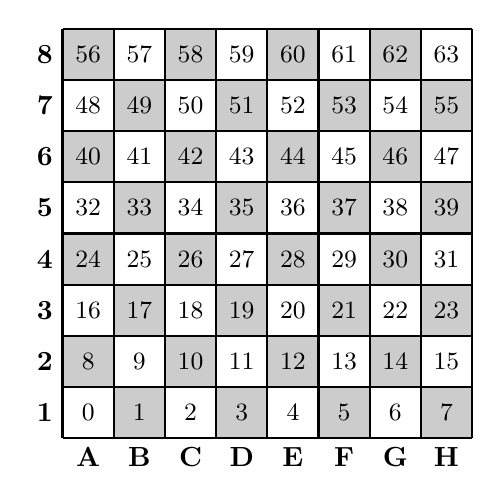
\begin{tikzpicture}[scale=0.65]
        % Draw the chessboard
        \foreach \x in {0,1,...,7} {
            \foreach \y in {0,1,...,7} {
                \pgfmathparse{mod(\x+\y,2) ? "black!20" : "white"}
                \edef\col{\pgfmathresult}
                \fill[\col] (\x,\y) rectangle (\x+1,\y+1);
                
                % Calculate the square index
                \pgfmathtruncatemacro{\num}{\x + 8*\y}
                % Add the number to the square
                \node at (\x+0.5,\y+0.5) {\small \num};
            }
        }

        % Add column labels (A-H)
        \foreach \x [count=\i from 0] in {A, B, C, D, E, F, G, H} {
            % \node[above] at (\i+0.5, 8) {\textbf{\x}}; % Top labels
            \node[below] at (\i+0.5, 0) {\textbf{\x}}; % Bottom labels
        }

        % Add row labels (1-8)
        \foreach \y [count=\i from 0] in {1, 2, 3, 4, 5, 6, 7, 8} {
            \node[left] at (0, \i+0.5) {\textbf{\y}}; % Left labels
            % \node[right] at (8, \i+0.5) {\textbf{\y}}; % Right labels
        }

        % Draw the grid
        \draw[thick] (0,0) grid (8,8);
    \end{tikzpicture}
    \caption{Little-Endian Rank-File Mapping with Coordinates.}
    \label{fig:lerf}
\end{figure}

\noindent \parbox{\textwidth}{There are bitboards for all pieces (\texttt{bitboard\_all}), for each piece color (\texttt{bitboard\_color[0]} and \texttt{bitboard\_color[1]}), and for each piece type (\texttt{bitboard\_piece[Piece]} like \texttt{bitboard\_piece[Piece::W\_QUEEN]})}.

\vspace{1em}

\noindent To identify ray directions on the board, we used the compass rose:

\begin{center}
    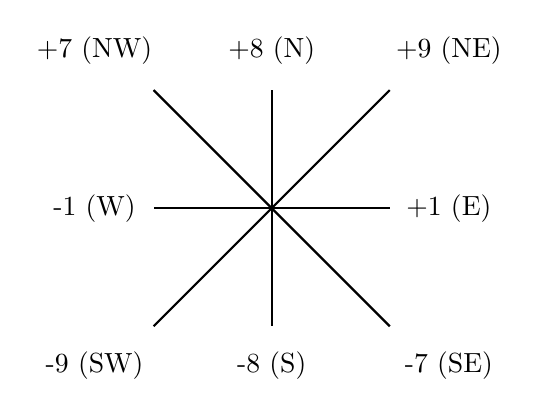
\begin{tikzpicture}
        \node at (0, 2) {+8 (N)};
        \node at (2.25, 2) {+9 (NE)};
        \node at (-2.25, 2) {+7 (NW)};
        \node at (2.25, 0) {+1 (E)};
        \node at (-2.25, 0) {-1 (W)};
        \node at (0, -2) {-8 (S)};
        \node at (2.25, -2) {-7 (SE)};
        \node at (-2.25, -2) {-9 (SW)};
        \draw[thick] (0, 0) -- (0, 1.5);
        \draw[thick] (0, 0) -- (1.5, 1.5);
        \draw[thick] (0, 0) -- (-1.5, 1.5);
        \draw[thick] (0, 0) -- (1.5, 0);
        \draw[thick] (0, 0) -- (-1.5, 0);
        \draw[thick] (0, 0) -- (0, -1.5);
        \draw[thick] (0, 0) -- (1.5, -1.5);
        \draw[thick] (0, 0) -- (-1.5, -1.5);
    \end{tikzpicture}
\end{center}

\noindent This means that, to get the numerical value that identifies the square to the north-east of a given square, you only need to add 9. For example, given the square $f6$ (45), the north-east square $g7$ has a value of 54 (45 + 9 = 54). It is really effective for sliding pieces to calculate their attacks.

\subsubsection{Transposition table}

The transposition table contains a list of entries. These entries are defined as a storage of information about a specific chess position, including its Zobrist key, evaluation score, best move, node type, and search depth.

\ldots

\subsubsection{History}

\ldots

\subsubsection{Move generator information}

\ldots

\subsection{Precomputed data}

Some tables are memory initialized instead of computed, explain it.

\ldots

\section{Additional tools and work}

\ldots

\subsection{Board visualizer using Python}

\ldots

\subsection{Profiling}

Continue in next Chapter~\ref{cap:profiling}.

\ldots

\subsection{Testing engine strength}

Testing and analysis in Chapter~\ref{cap:testing}.

\ldots